\documentclass[]{report}
\usepackage{amsmath}
\usepackage{graphicx}
\usepackage{tabularx}
\usepackage{amsfonts}
\usepackage{amssymb}
\usepackage{amsbsy}

% Title Page
\title{MachineLearning for Visual Computing Aufgabenblock 1}
\author{Christian Br\"andle}


\begin{document}
\maketitle

\begin{abstract}
\end{abstract}

\section{Einfaches Perceptron - Datengeneration}

% Mu_1 = [14,14,14,14]; 
% Sigma_1 = [5,4,3,2];
% Mu_2 = [2, 2, 2, 2]; 
% Sigma_2 = [2,3,4,5];

Gegeben sind vier Datensets a 100 Beobachtungen von 2-dimensionalen Eingangsdaten, welche normalverteilt sind. Die Figuren in Tabelle ~\ref{tab:DataSets} verdeutlichen dies.


\begin{table}[h]
\begin{tabular}{| c | c |}
\hline
 & \\
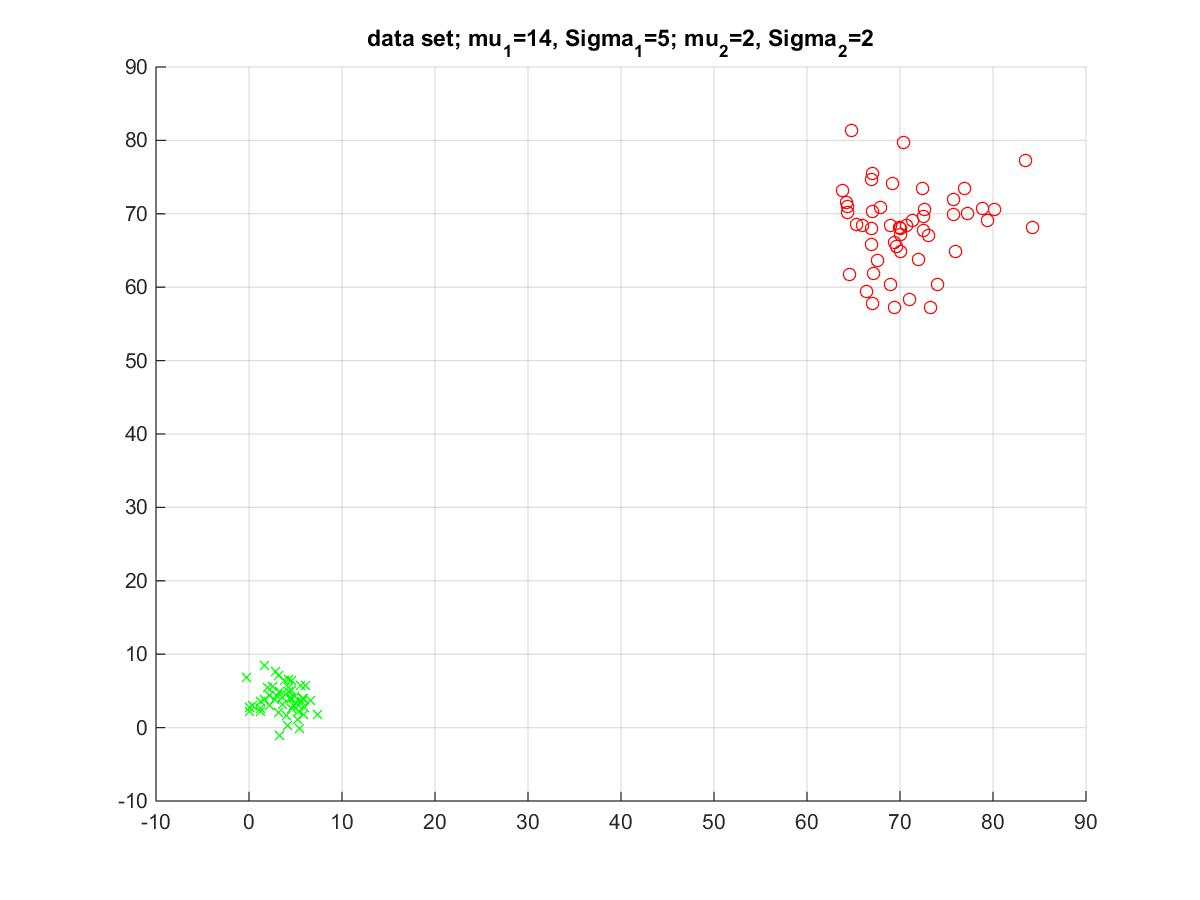
\includegraphics[width=0.4\textwidth]{./images/DataSet_100.jpg} & 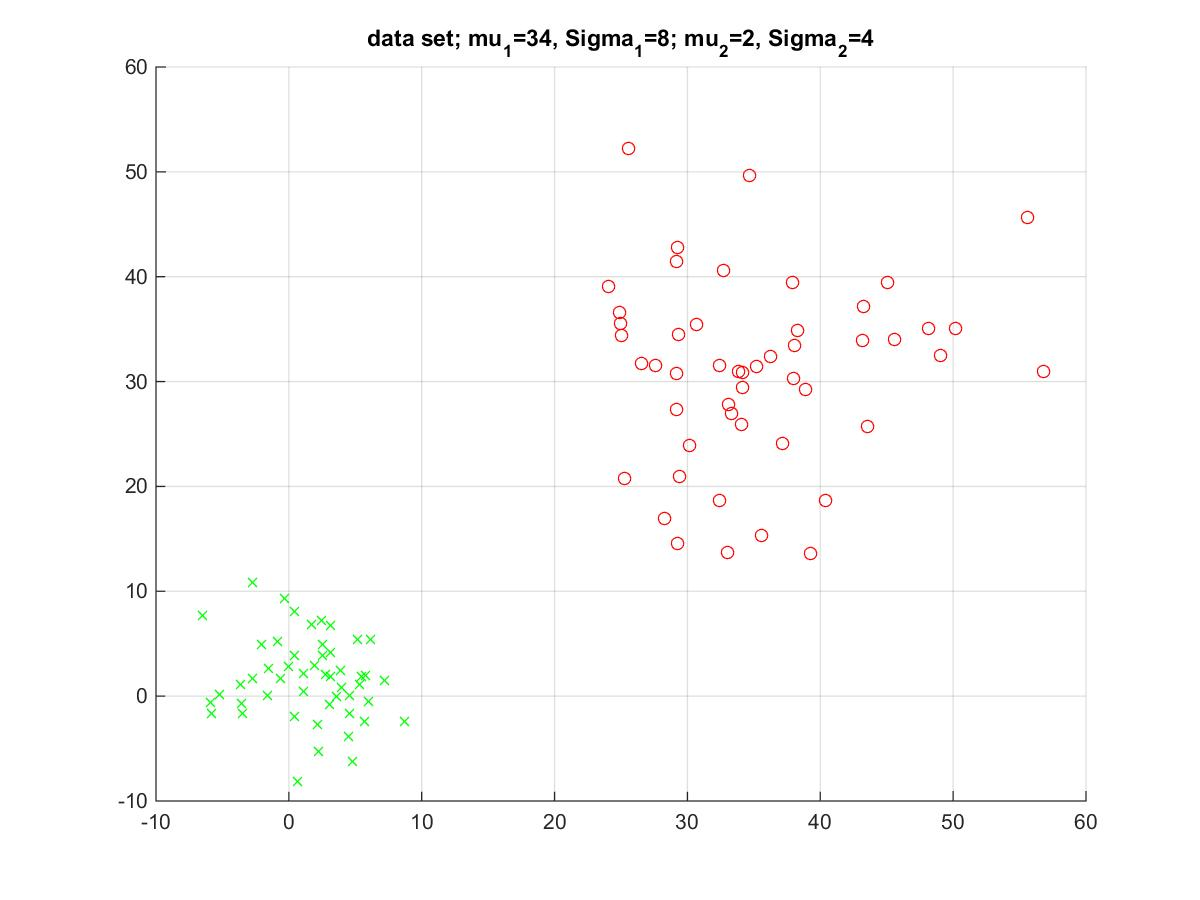
\includegraphics[width=0.4\textwidth]{./images/DataSet_200.jpg} \\
 & \\
\hline
 & \\
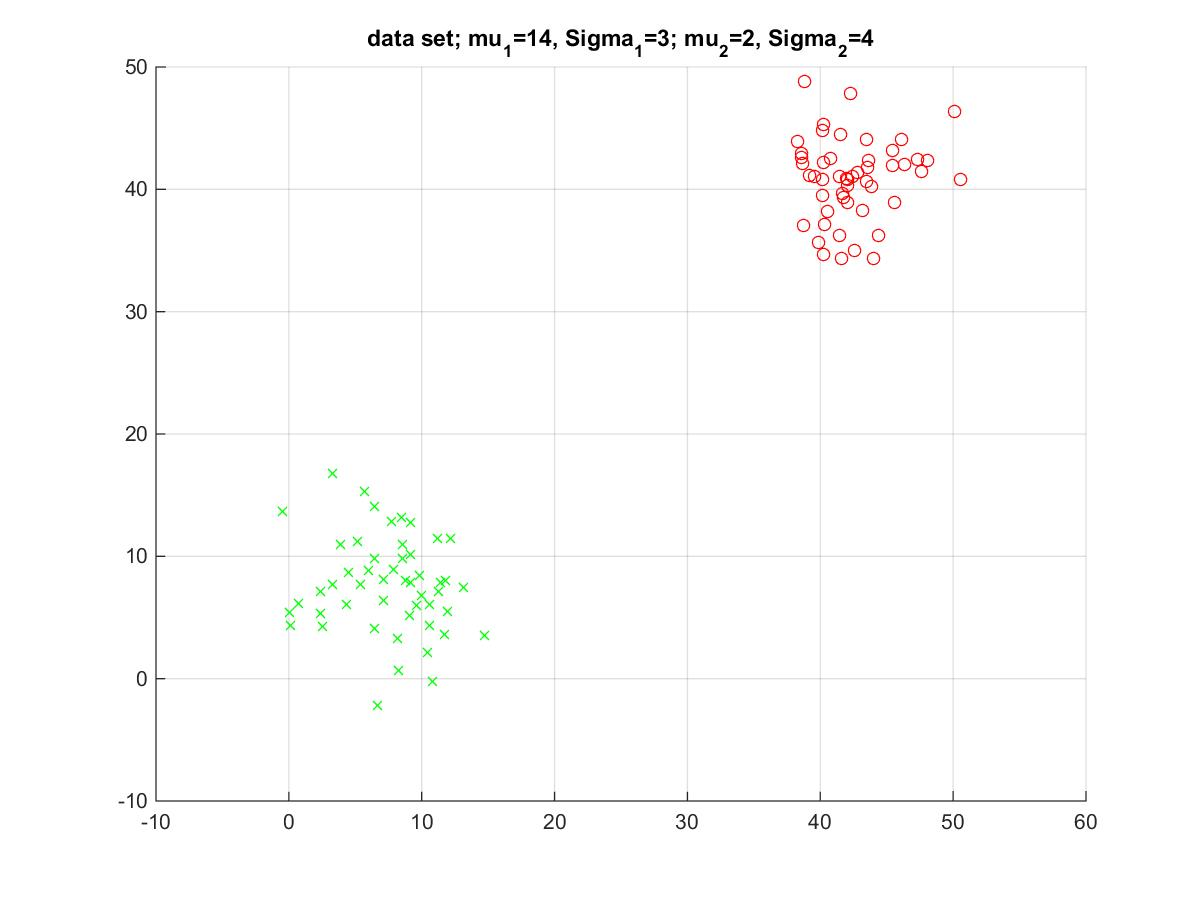
\includegraphics[width=0.4\textwidth]{./images/DataSet_300.jpg} & 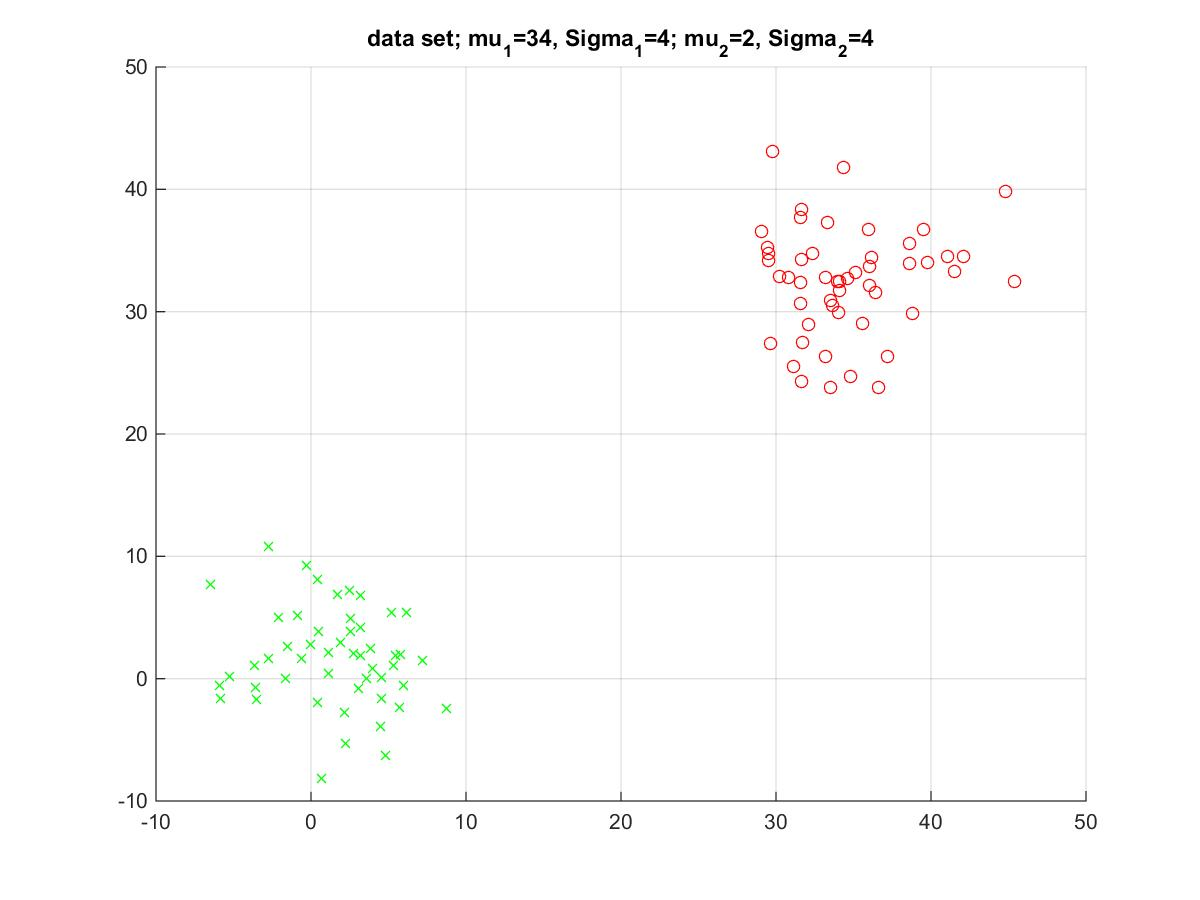
\includegraphics[width=0.4\textwidth]{./images/DataSet_400.jpg} \\
 & \\
\hline
\end{tabular}
\caption{Iteration distribution over gamma}
\label{tab:DataSets}
\end{table}

\section{Einfaches Perceptron - Perceptrontraining}

\subsection{Anzahl Iterationen}

Die Anzahl der Iterationen h\"angt ma{\ss}geblich von der \emph{margin} der separierbaren Daten ab. Je kleiner die margin, desto mehr Iterationen sind notwendig, bis der Algorithmus terminiert.


\subsection{Welchen Einflu{\ss} hat die Schrittweite}

Der Einflu{\ss} der Schrittweite h\"angt sowohl von den Eingangsdaten als auch vom gew\"ahlten Algorithmus ab.
Es ist zu beobachten, da{\ss} der batch-Algorithmus keine gro{\ss}en Abweichungen zeigt, egal welches $\gamma$ gew\"ahlt wird. Beim online-Verfahren ist der Einflu{\ss} gr\"o{\ss}er, das hei{\ss}t die Varianz in den ermittelten Iterationen ist h\"oher, aber auch hier ist kein eindeutiger Bereich \"uber alle Simulationen auszumachen, wo ein gegebenes $\gamma$ die Iterationen des Algorithmus wesentlich reduziert.

\begin{table}[h]
\begin{tabular}{| c | c |}
\hline
 & \\
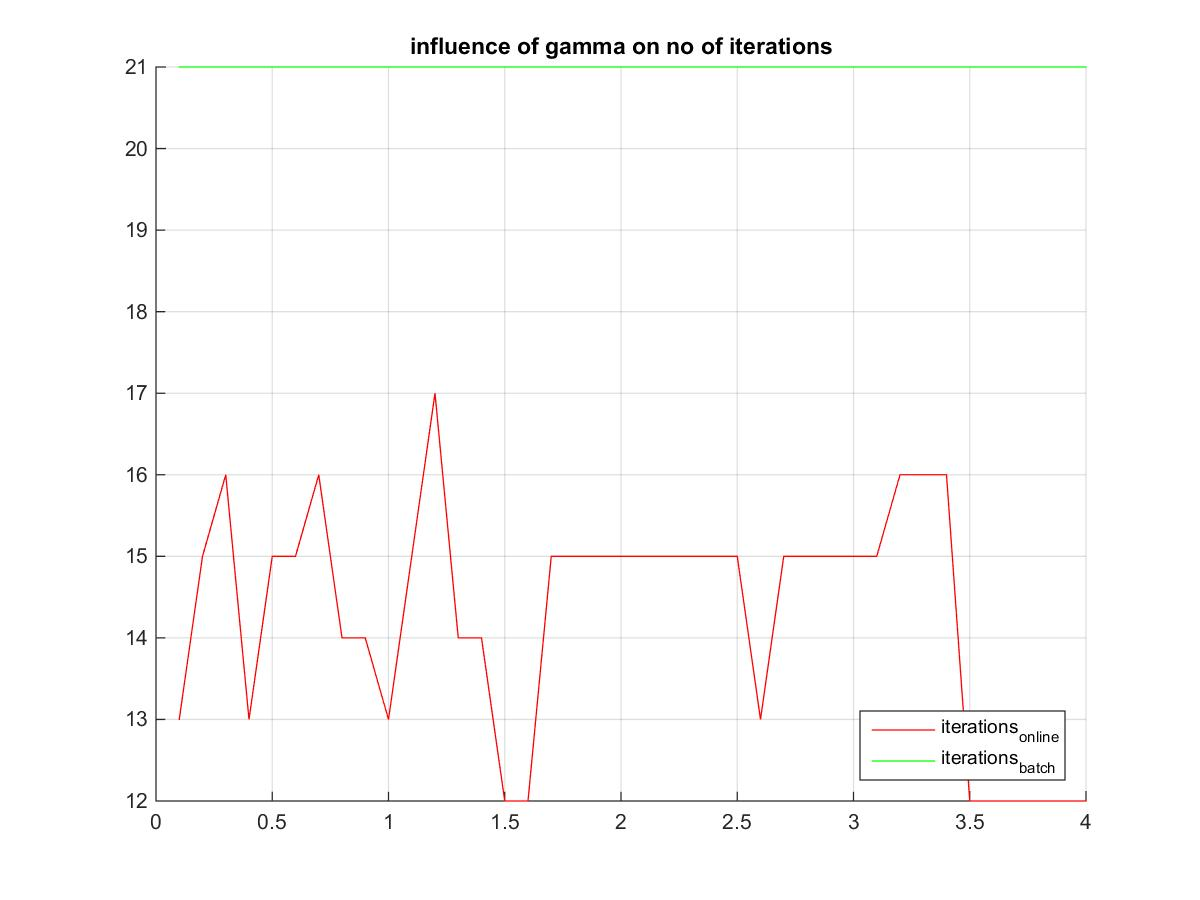
\includegraphics[width=0.4\textwidth]{./images/GammaToIterations_0150.jpg} & 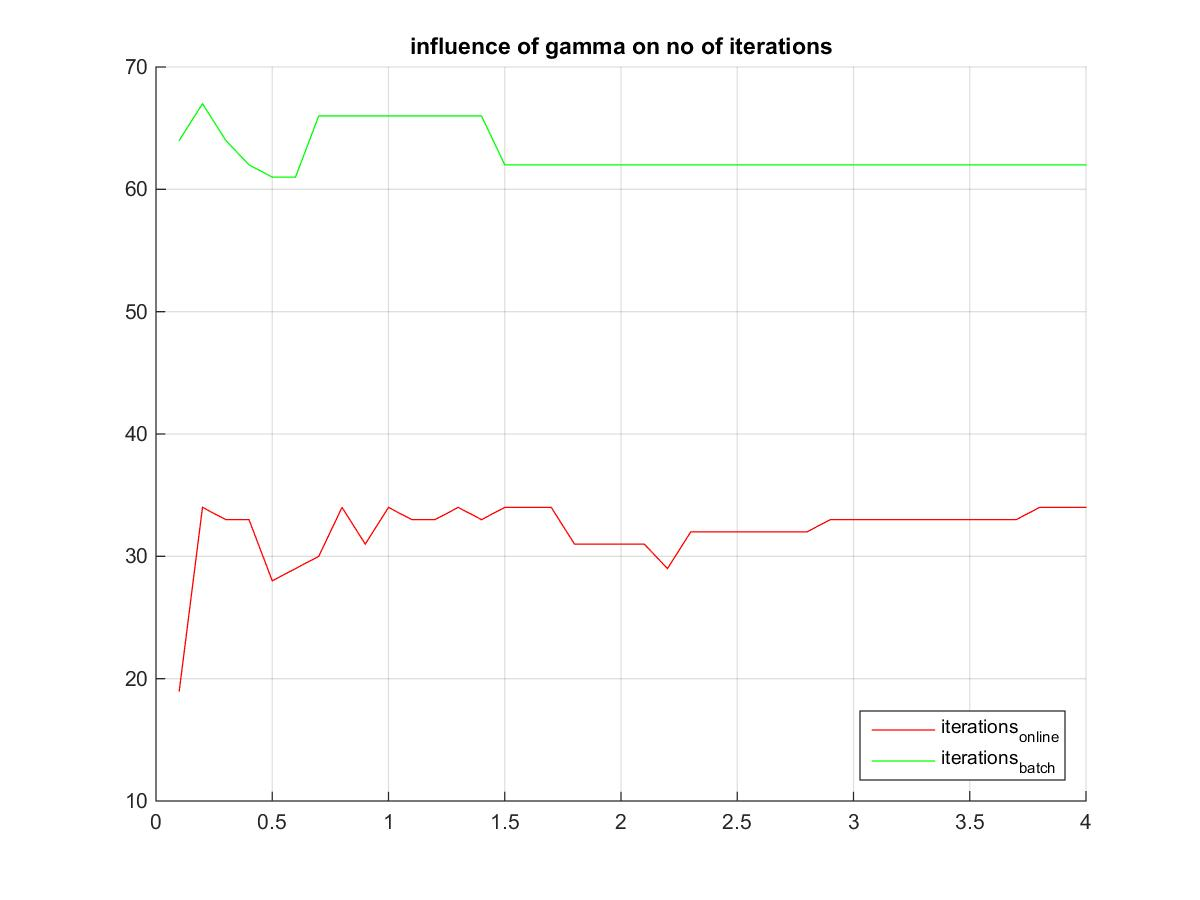
\includegraphics[width=0.4\textwidth]{./images/GammaToIterations_0250.jpg} \\
 & \\
\hline
 & \\
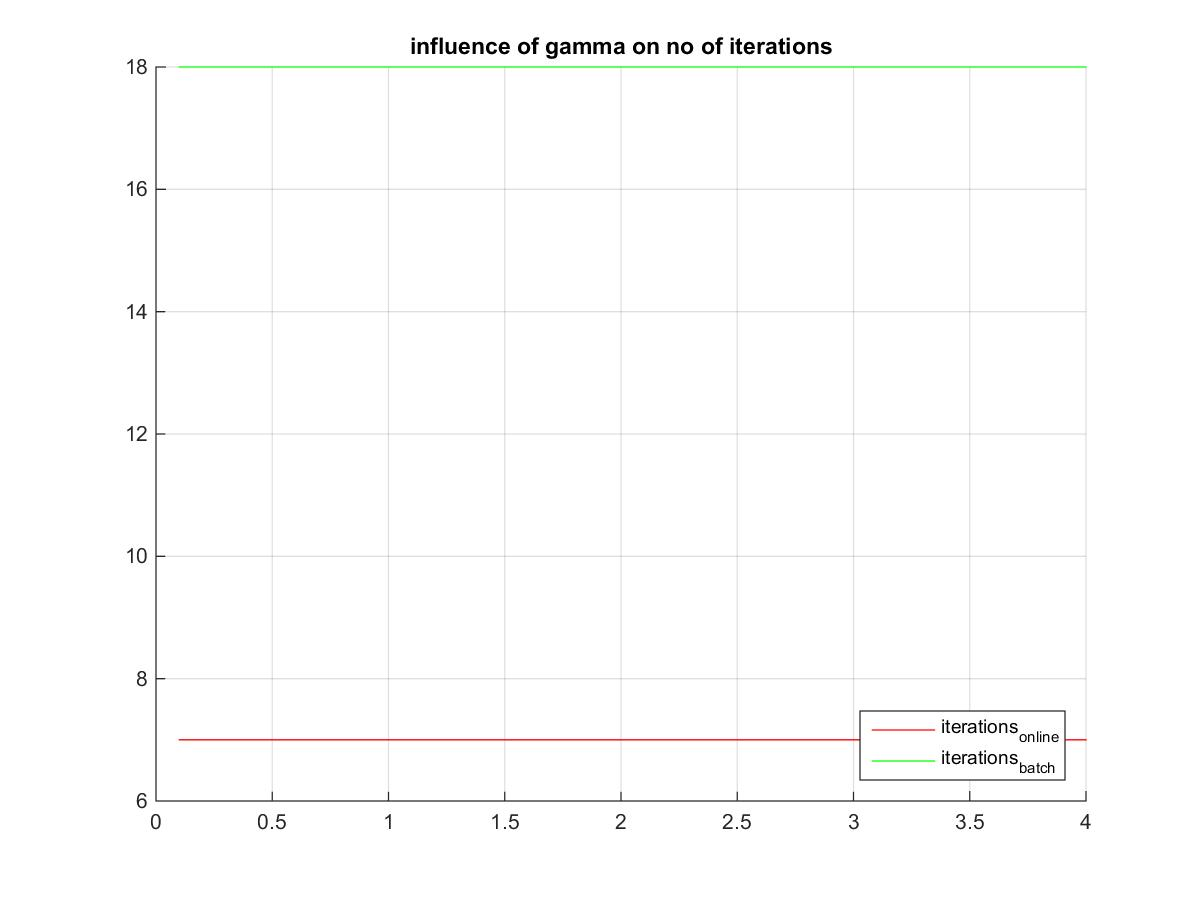
\includegraphics[width=0.4\textwidth]{./images/GammaToIterations_0350.jpg} & 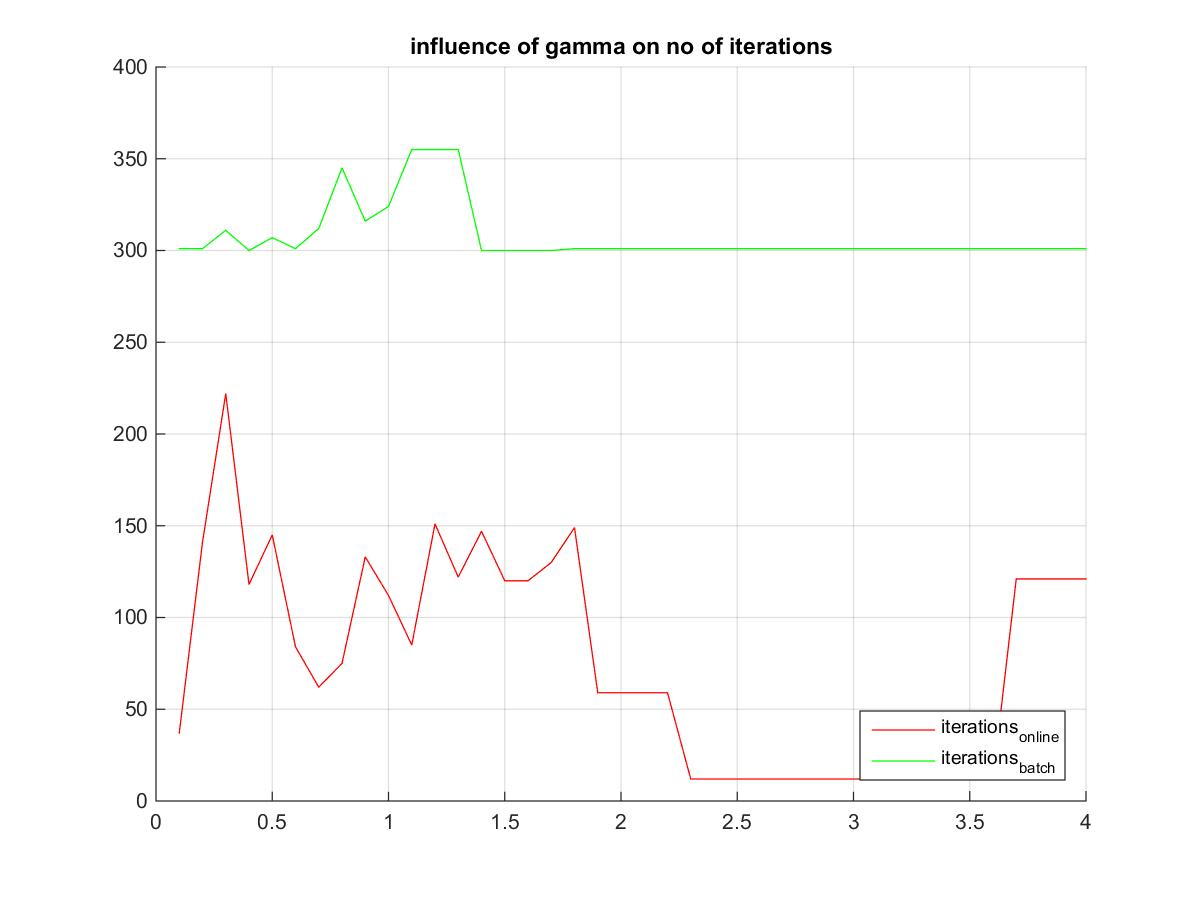
\includegraphics[width=0.4\textwidth]{./images/GammaToIterations_0450.jpg} \\
 & \\
\hline
\end{tabular}
\caption{Iteration distribution over gamma}
\label{tab:GammaToIterations}
\end{table}


\subsection{Daten und Entscheidungsgrenzen im $\mathbb{R}^2$}


\begin{table}[h]
\begin{tabular}{| c | c |}
\hline
 & \\
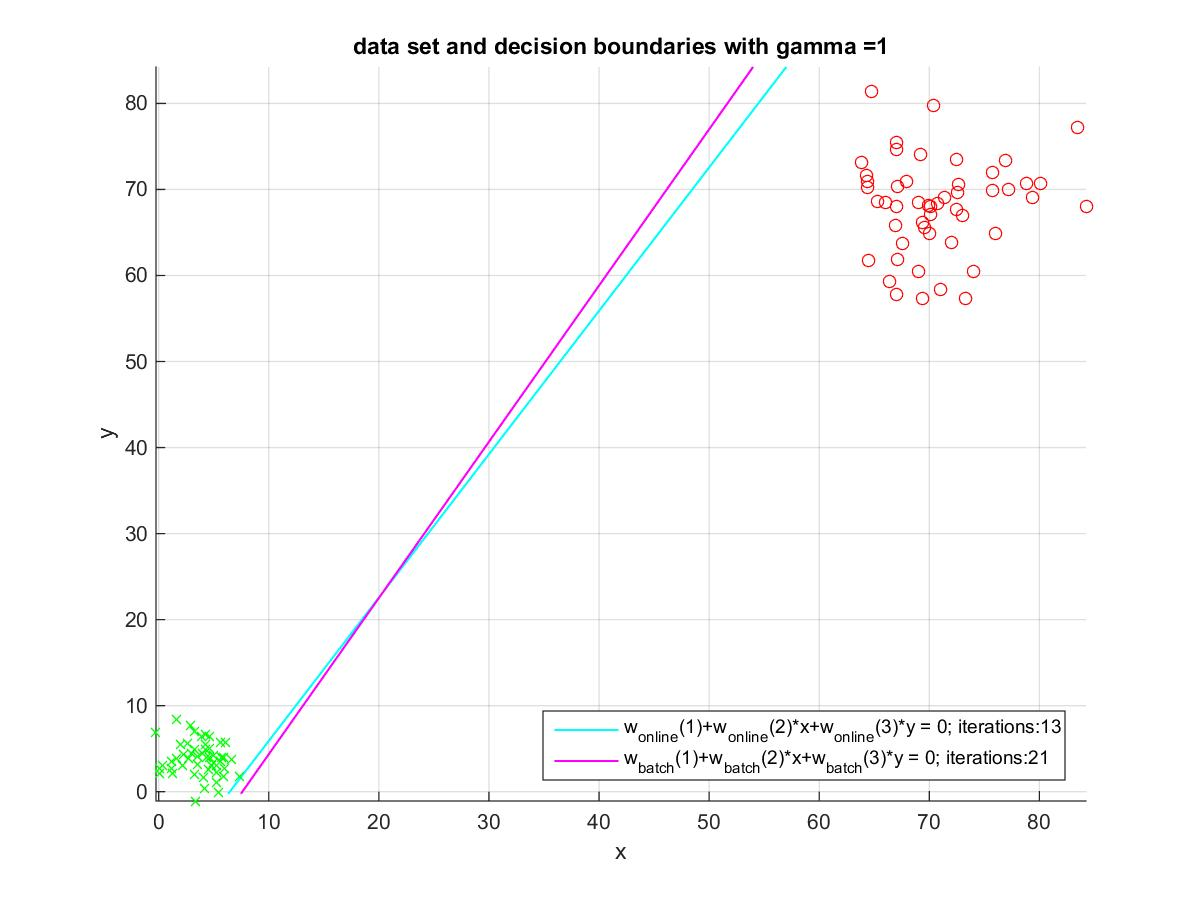
\includegraphics[width=0.4\textwidth]{./images/DataSetAndDecisionBoundary_110.jpg} & 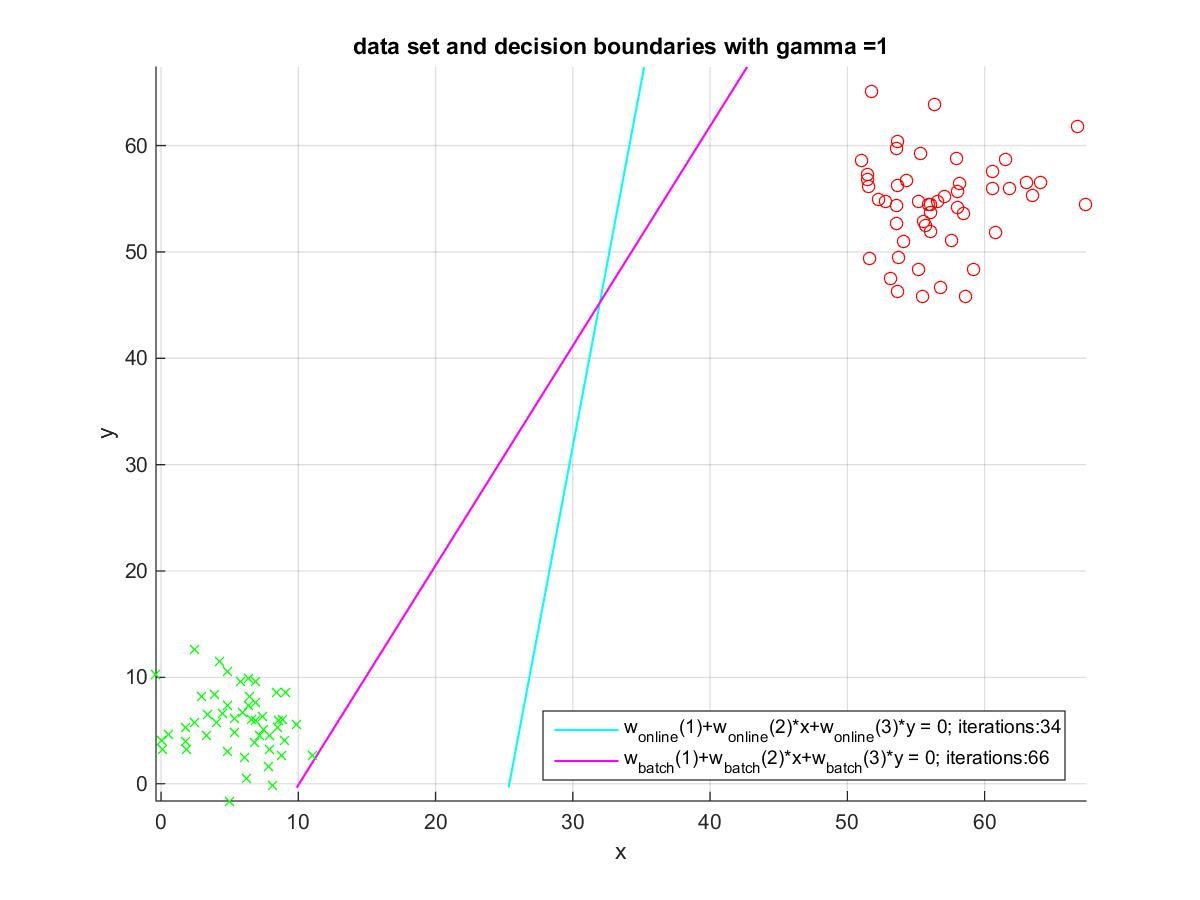
\includegraphics[width=0.4\textwidth]{./images/DataSetAndDecisionBoundary_210.jpg} \\
 & \\
 $set_{1}$: $\mu_1=10$, $\Sigma_1=5$ & $set_{1}$: $\mu_1=10$, $\Sigma_1=4$ \\
 $set_{2}$: $\mu_2=2$, $\Sigma_2=2$ & $set_{2}$: $\mu_2=2$, $\Sigma_2=3$ \\
\hline
 & \\
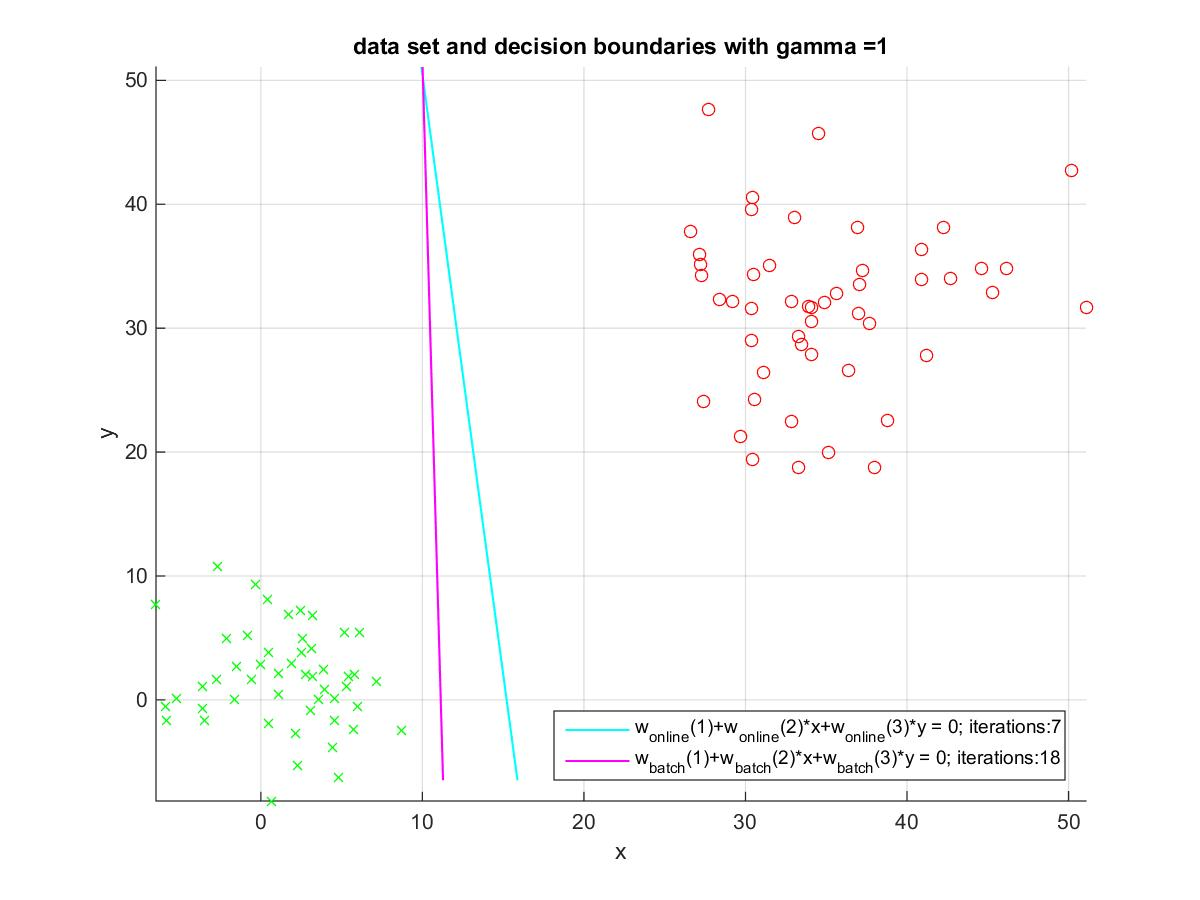
\includegraphics[width=0.4\textwidth]{./images/DataSetAndDecisionBoundary_310.jpg} & 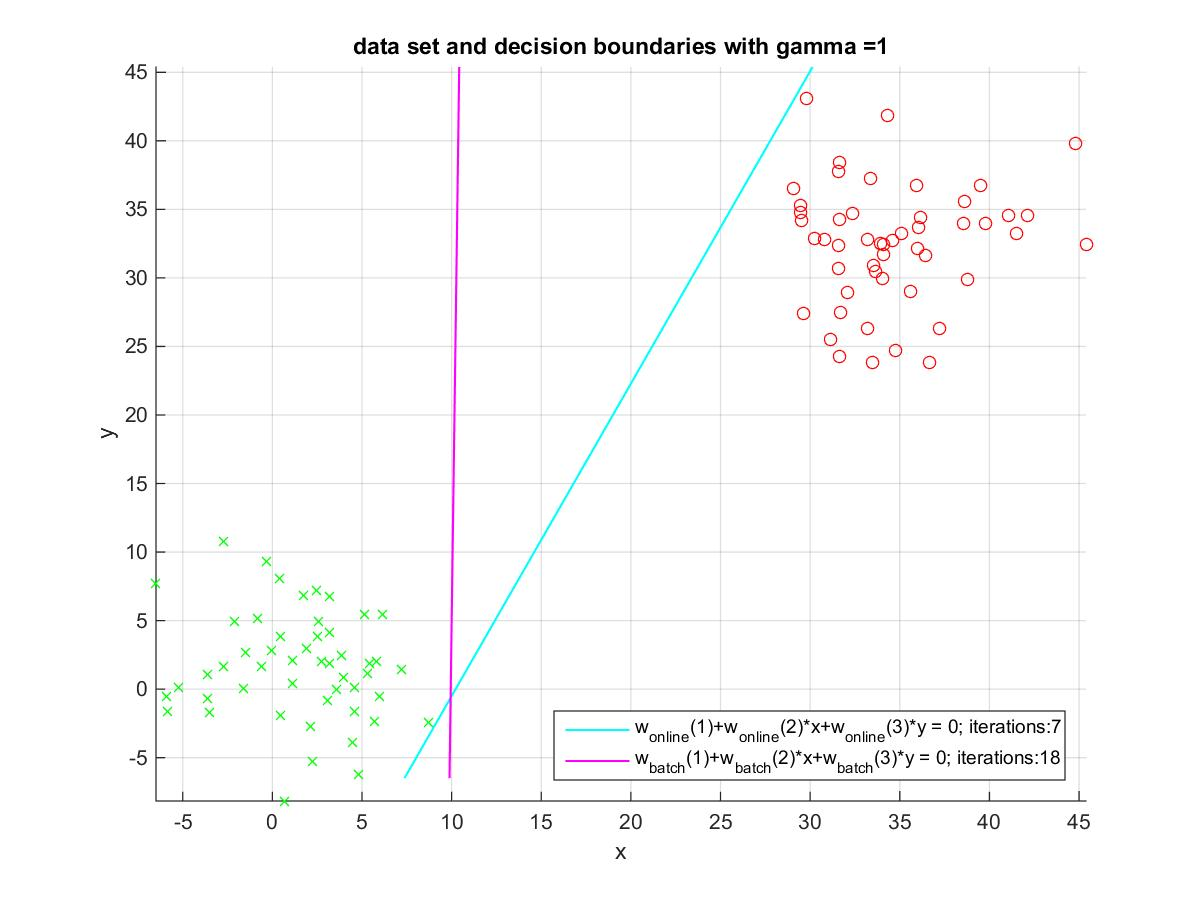
\includegraphics[width=0.4\textwidth]{./images/DataSetAndDecisionBoundary_410.jpg} \\
 & \\
$set_1$: $\mu_1=10$, $\Sigma_1=3$ & $set_1$: $\mu_1=10$, $\Sigma_1=2$ \\
$set_2$: $\mu_2=2$, $\Sigma_2=4$ & $set_2$: $\mu_2=2$, $\Sigma_2=5$ \\
\hline
\end{tabular}
\caption{Iteration distribution over gamma}
\label{tab:DataSetsAndBounds}
\end{table}


\subsection{Wie ist das Verhalten bei nicht linear separierbaren Daten}

Der Algorithmus terminiert nicht da bei jedem Durchlauf Daten gefunden werden, welche in der falschen Klasse landen.

\end{document}          
